\subsection{Sprint 3}

Στην ενότητα αυτή παρουσιάζονται οι τιμές των μετρικών που
χρησιμοποιήθηκαν για κάθε κλάση/enumeration στο τέλος του sprint 3, το
οποίο σημαδεύει και το τέλος της ανάπτυξης του συστήματος. Οι
βασικότερες αλλαγές που πραγματοποιήθηκαν κατά τη διάρκεια του sprint 3
είναι η προσθήκη λειτουργικότητας κόστους και πληρωμών για τις
κρατήσεις, η προσθήκη κλάσεων για τη διαχείριση των τύπων δωματίων
και η αλλαγή του τρόπου παρουσίασης των στοιχείων για τα διαφορετικά
τμήματα λειτουργικότητας της εφαρμογής, όπως η διαχείριση χρηστών,
δωματίων κλπ. Αυτό είχε ως αποτέλεσμα την προσθήκη ακόμα περισσότερων
βοηθητικών κλάσεων διεπαφής αλλά και λίγων κλάσεων με λετουργικότητα
backend.

\subsubsection{Logical Lines Of Code (LLOC)}
\label{section:sprint3LLOC}

Στο σχήμα \ref{fig:sprint3LLOC} εμφανίζεται ο αριθμός των λογικών
γραμμών κώδικα για κάθε κλάση στο τέλος του sprint 3. Παρατηρούμε ότι η
κλάση DBManager είναι εκ νέου αυτή με το μεγαλύτερο μέγεθος, αφού σε
αυτή προστέθηκαν λειτουργίες για τη διαχείριση της βάσης δεδομένων
σχετικές με το κόστος και τις πληρωμές των κρατήσεων αλλά και των τύπων
δωματίων. Το μέγεθος της κλάσης πιθανόν να αρχίζει να γίνεται μη
εύκολα διαχειρίσιμο πια και θα ήταν σίγουρα προτιμότερο να διασπαστεί σε
μικρότερες κλάσεις, η κάθε μία από τις οποίες θα διαχειρίζεται την
επικοινωνία με τη βάση δεδομένων σχετικά μόνο με ένα τύπο δεδομένων.

\begin{figure}
\centering
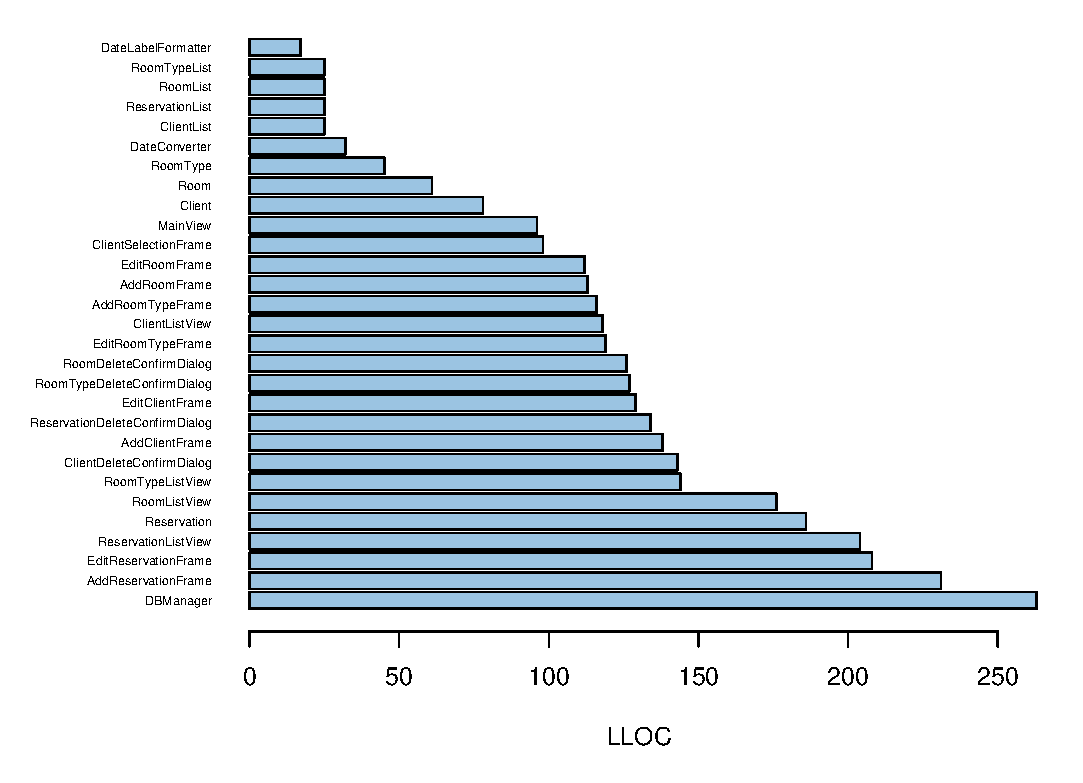
\includegraphics[width=1.0\textwidth]{Sprint3-LLOC-1.eps}
\caption{Λογικές γραμμές κώδικα ανά κλάση στο τέλος του sprint 3}
\label{fig:sprint3LLOC}
\end{figure}

Οι υπόλοιπες κλάσεις με σχετικά μεγάλο μέγεθος είναι οι κλάσεις γραφικής
διασύνδεσης που διαχειρίζονται τις κρατήσεις. Όπως αναφέρθηκε
προηγουμένως στη συζήτηση των τιμών των μετρικών κατά τη διάρκεια του
sprint 2, οι περισσότερες από αυτές θα μπορούσαν πιθανόν να διασπαστούν
σε μικρότερες κλάσεις.

\subsubsection{Clone Coverage (CC)}
\label{section:sprint3CC}

Το σχήμα \ref{fig:sprint3CC} εμφανίζει τις τιμές της μετρικής επανάληψης
κώδικα CC για κάθε κλάση στο τέλος του sprint 3. Όπως και στο αντίστοιχο
σχήμα για το sprint 2, και σε αυτή την περίπτωση οι κλάσεις με τις
μεγαλύτερες τιμές είναι με διαφορά οι κλάσεις γραφικής διασύνδεσης. Όπως
και στα αντίστοιχα αποτελέσματα του sprint 2, η επανάληψη κώδικα σε
αυτές τις κλάσεις οφείλεται κυρίως στον κώδικα που έχει παραχθεί
αυτόματα με το σχεδιασμό και την τοποθέτηση των διάφορων γραφικών
συστατικών όπως κουμπιά, λίστες κλπ στα αντίστοιχα παράθυρα.

\begin{figure}
\centering
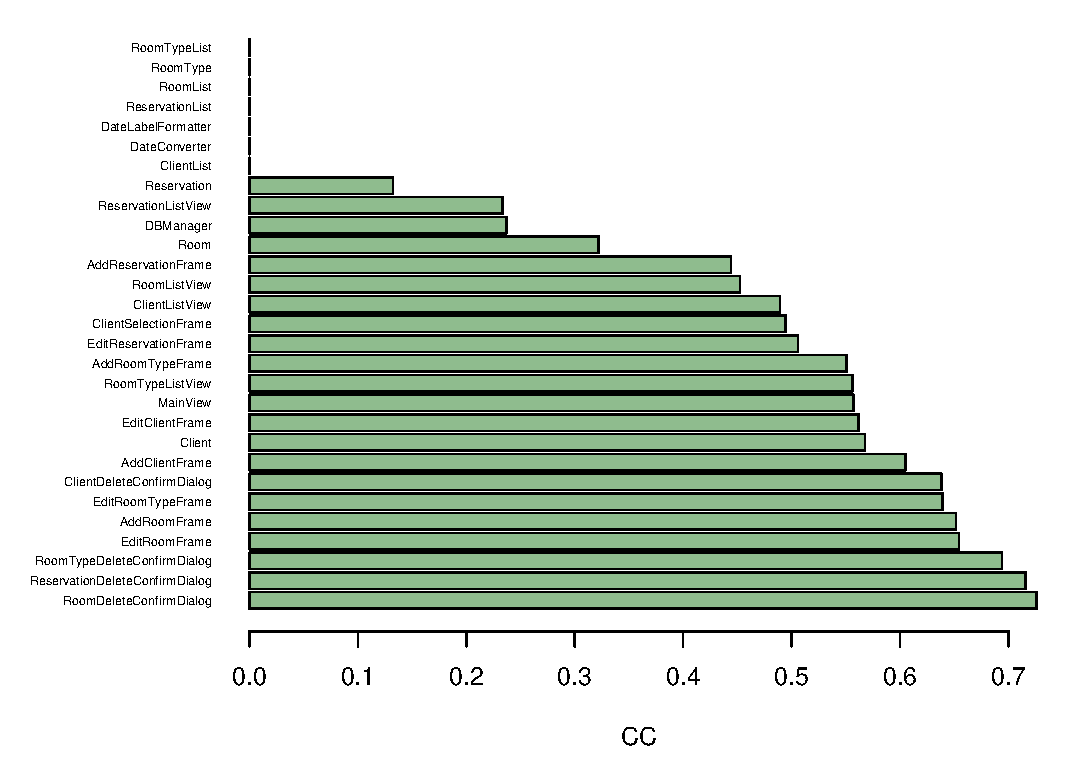
\includegraphics[width=1.0\textwidth]{Sprint3-CC-1.eps}
\caption{Τιμές της μετρικής CC ανά κλάση στο τέλος του sprint 3}
\label{fig:sprint3CC}
\end{figure}

Για τις κλάσεις backend με υψηλές τιμές, όπως η κλάση Client ισχύουν τα
όσα ειπώθηκαν στην ενότητα \ref{section:sprint1CC}, με την
επαναληψιμότητα να οφείλεται σε κώδικα ελέγχου της μεθόδου main και ο
οποίος ουσιαστικά δεν επηρεάζει την λειτουργία του συστήματος στο
παραμικρό.



\subsubsection{McCabe’s Cyclomatic Complexity (McCC)}
\label{section:sprint3McCC}

\begin{figure}
\centering
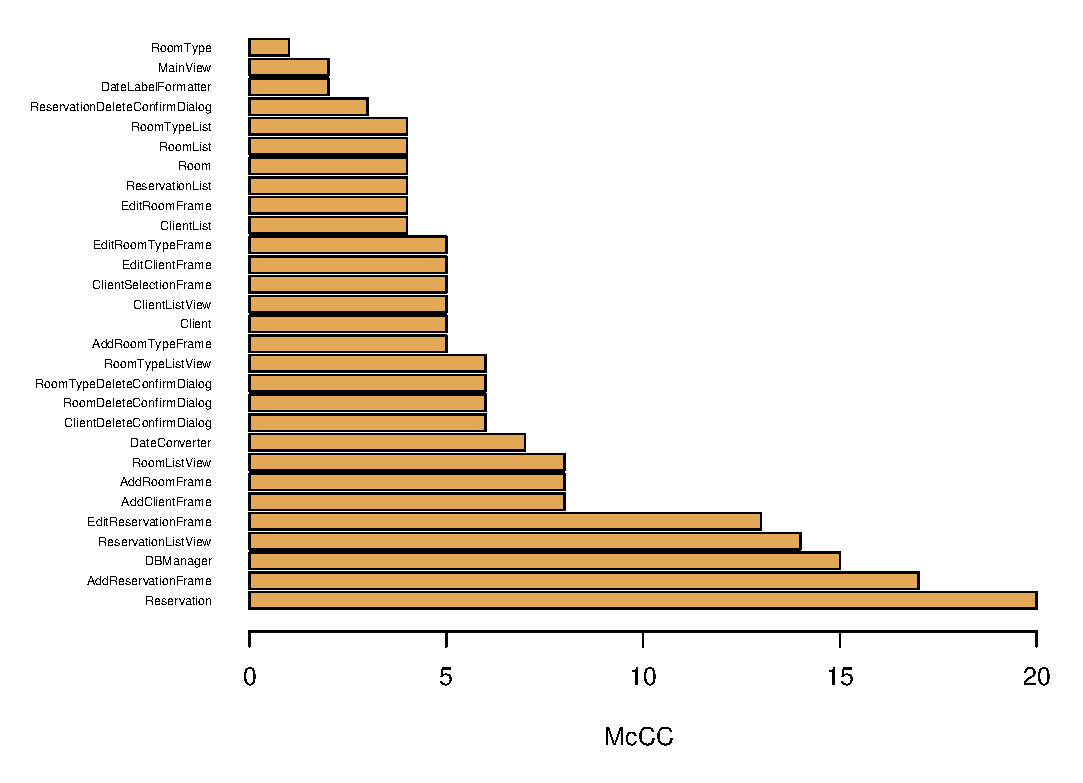
\includegraphics[width=1.0\textwidth]{Sprint3-McCC-1.eps}
\caption{Τιμές της μετρικής κυκλωματικής πολυπλοκότητας McCC ανά κλάση στο τέλος του sprint 3}
\label{fig:sprint3McCC}
\end{figure}

\subsubsection{Lack of Cohesion in Methods 5 (LCOM5)}
\label{section:sprint3LCOM5}

\begin{figure}
\centering
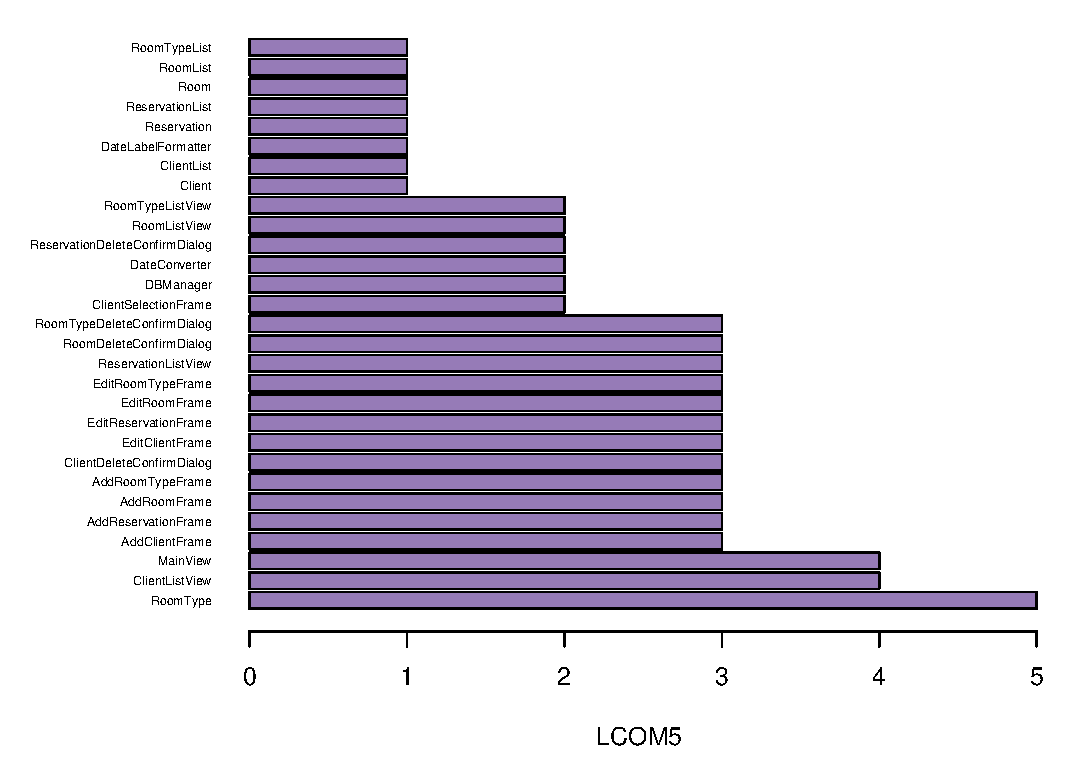
\includegraphics[width=1.0\textwidth]{Sprint3-LCOM5-1.eps}
\caption{Τιμές της μετρικής έλλειψης συνεκτικότητας LCOM5 ανά κλάση στο τέλος του sprint 3}
\label{fig:sprint3LCOM5}
\end{figure}

\subsubsection{Coupling Between Object classes (CBO)}
\label{section:sprint3CBO}

\begin{figure}
\centering
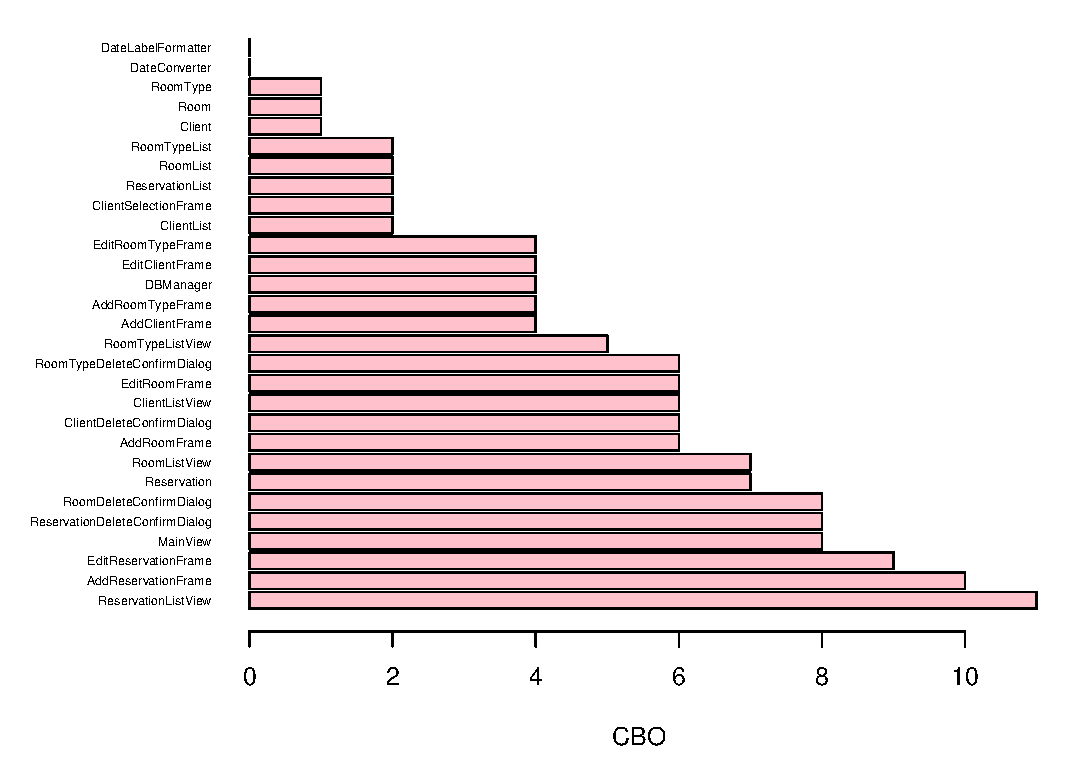
\includegraphics[width=1.0\textwidth]{Sprint3-CBO-1.eps}
\caption{Τιμές της μετρικής σύζευξης CBO ανά κλάση στο τέλος του sprint 3}
\label{fig:sprint3CBO}
\end{figure}
